%!TEX root = main.tex

%%%%%%%%%%%%%%%%%%%%%%%%%%%%%%%%%%%%%%%%%%%%%%%%%%%%%%%%%%%%%%%%%%
\chapter{TorMentor Design}
\label{sec:design}
%%%%%%%%%%%%%%%%%%%%%%%%%%%%%%%%%%%%%%%%%%%%%%%%%%%%%%%%%%%%%%%%%%

TorMentor design has three goals: (1) meet the defined learning
objective in a reasonable amount of time, (2) provide both anonymity
and data privacy guarantees to clients and curators, and (3) flexibly
support client-specific privacy requirements.

\section{Design overview}

The broker handles all communication between
clients and the curator, and acts as the coordinator in an untrusted
collaborative learning setting. Each TorMentor broker is deployed as a
Tor hidden service with a unique and known \textit{.onion}
domain. Several clients may join a model once a curator defines it,
with requirements for joining specified by both the curator and the
clients. Each broker and therefore each model is associated with a pool
of clients among whom the learning procedure takes place (see 
Figure~\ref{fig:sysdiagram}).

Each broker runs a separate \emph{aggregator} process and 
\emph{validator} process. The aggregator serves the same purpose as a
parameter server~\cite{Li:2014}: storing and distributing the
parameters of the global model. The validator is a novel addition in
our work that observes and validates the values of gradient updates
sent by clients to the aggregator.

Next, we review the TorMentor curator and client \ac{API} in 
Tables~\ref{tab:CurAPI} and~\ref{tab:CliAPI}. We also review the
training process illustrated in Figure~\ref{fig:protocol}, and finally
detail how TorMentor defends against adversarial clients and curators.

\section{Curator API}

\begin{table}[t]
\begin{tabular}{p{\textwidth}}
% return-val $\leftarrow$ call(args)} 
 %\textbf{API call}                                                 & 
 %\textbf{Description}                                                                 \\
 \hline \hline
 address $\leftarrow$ \textbf{curate}(mID, maxCli, minCli, validSet) \\
 \hline
 Curate a new model. Curator provides modelID,  
 client count range, validation set. TorMentor returns a hidden
 service address for a newly specified broker. \\
 \hline
\end{tabular} 
\caption{TorMentor Curator API.\label{tab:CurAPI} }
\end{table}

\begin{table}[t]
\begin{tabular}{p{\textwidth}}
 \hline \hline
 $P_{admit}$ $\leftarrow$ \textbf{join}(mID) \\
 \hline
 Client joins a curated model. Client provides modelID; TorMentor returns
 a SHA-256 admission hash puzzle $P_{admit}$.                          
 \\
 \hline \hline
 conn, $M_t$ $\leftarrow$ \textbf{solve}(mID, $S_{admit}$, minCli, schema) \\
 \hline
 Client finds the solution $S_{admit}$ to $P_{admit}$ and joins. Client
 provides modelID, solution to puzzle, min number of clients and its
 dataset schema; TorMentor returns a connection and global model state.
 \\
 \hline \hline
 $M_{g,t+1}$, $P_{i,t+1}$ $\leftarrow$ \textbf{gradientUpdate}(mId, $S_
 {i,t}$, $\Delta_{i,t}$) \\
 \hline
 Client pushes a local model update to the global model state. Client $i$
 provides modelID, solution to previous SHA-256 puzzle $S_{i,t}$ and
 gradient update $\Delta_{i,t}$ at iteration $t$; TorMentor returns new
 global model state $M_{g,t+1}$, and the next SHA-256 puzzle $P_
 {i,t+1}$. \\
 \hline
\end{tabular} 
\caption{TorMentor Client API.\label{tab:CliAPI} }
\end{table}

Table~\ref{tab:CurAPI} shows the curator API in TorMentor. The curator
uses the \textbf{curate} call to bootstrap a new model by defining
a \emph{common learning objective}: the model type, the desired
training data schema and a validation dataset. These are critical to
perform ML successfully (even in a local setting). We therefore expect
that a curator can provide these.

Once the learning objective is defined, a Tor \textit{.onion} address
is established for the specified model, and the system waits for
clients to contact the hidden service with a message to join. The
validation dataset is used by the validator to reject adversaries, and
to ensure that the ML training is making progress towards model
convergence.

Too few clients may lead to a weak model with biased data, while a
large number of clients will increase communication overhead. The
curator can use the API to adjust an acceptable range for the number of
clients contributing to the model.

\section{Client API} 

Table~\ref{tab:CliAPI} shows the client API in TorMentor. 
A client uses the \textbf{join} call to join a curated model
\footnote{We assume that the client is able to learn the
curator-provided modelID out of band. This may be through a
third-party system or directly through another anonymous service.}. A
client's data is validated against the objective when joining. Our
prototype only checks that the specified number of features matches
those of the client, but more advanced automatic schema validation
techniques~\cite{Rahm:2001} can be used.

The client uses the \textbf{solve} call to perform a proof-of-work
validation, similar to that of the blockchain 
protocol~\cite{Nakamoto:2009}, in which a cryptographic SHA-256
admission hash is inverted, the solution is verified to contain
a required number of trailing `0' digits, and a new puzzle is
published. Once the proof-of-work is completed, the client is accepted
as a contributor to the model. Once the desired number of clients have
been accepted to the model, collaborative model training is performed
through the TorMentor protocol: each client computes their SGD update
on the global model and pushes it to the parameter server through the 
\textbf{gradientUpdate} call.

Clients compute gradient updates \emph{locally}. Clients also
maintain a personal privacy level $\varepsilon$ and a personal batch
size $b$ to tune their differentially-private updates during model
training. With the privacy-utility tradeoff in mind, it is natural for
clients and curators to have different preferences regarding client
privacy. Some clients may value privacy more than others and thus will
tune their own privacy risk, while curators want to maximize their
model utility \emph{TorMentor is the first system to support anonymous
machine learning in a setting with heterogeneous user-controlled
privacy goals.}

\section{Training process}
\label{sec:training}

\begin{figure}[t]
  \centering
  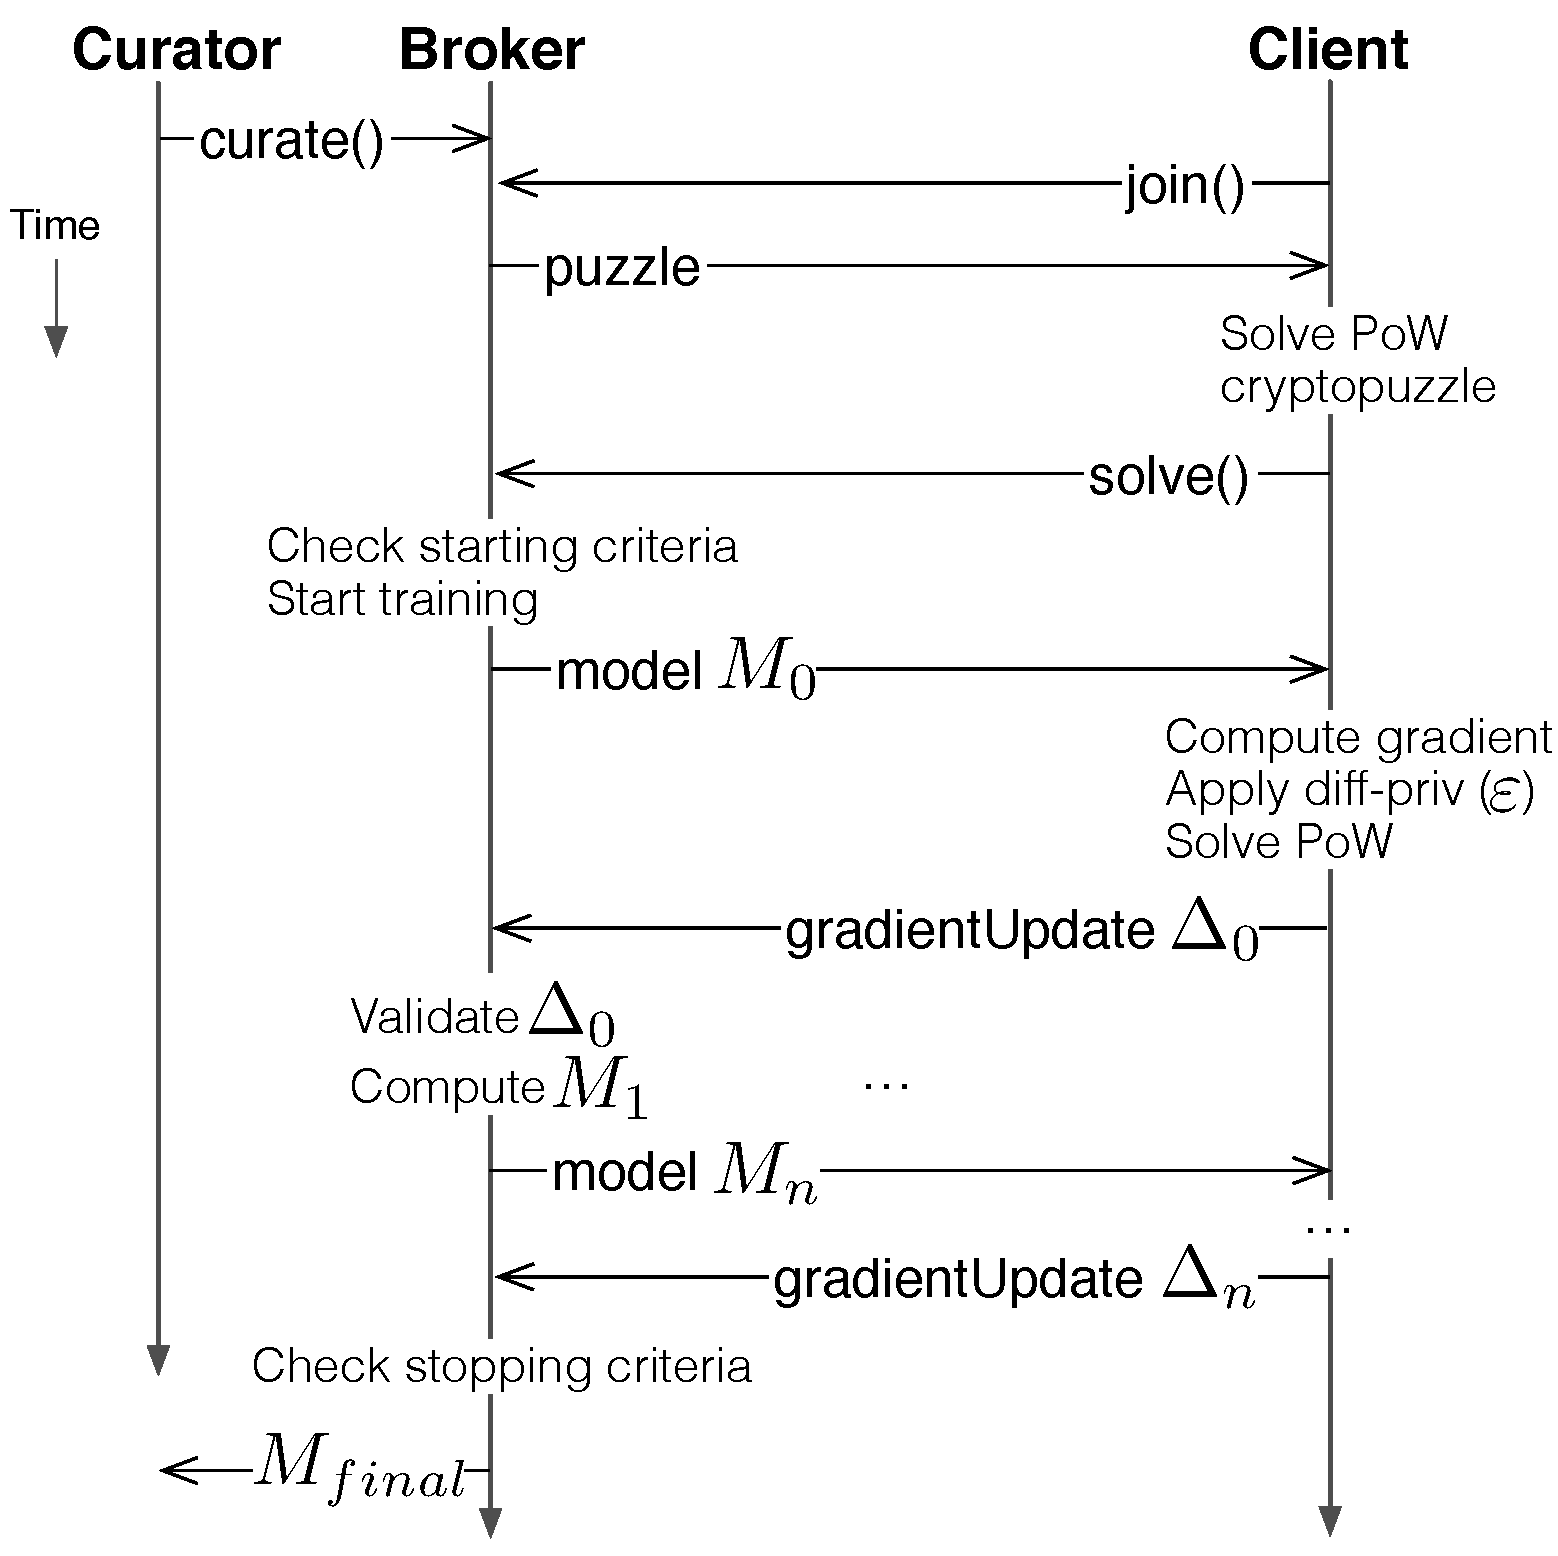
\includegraphics[width=.9\linewidth]{fig/tormentor-protocol.pdf}
  \caption{Overview of the TorMentor protocol between
    curator/broker/client.
    }
  \label{fig:protocol}
\end{figure}

Training in TorMentor (Figure~\ref{fig:protocol} and 
Algorithm~\ref{alg:training}) is performed in a
fashion similar to that of the parameter server~\cite{Li:2014}:
each client pulls the global model, locally computes a gradient step,
and applies the update to the global model. TorMentor uses the
differentially private SGD~\cite{Song:2013} method, which allows
clients to select their own privacy parameter $\varepsilon$ and batch
size $b$. We assume that clients understand how to properly define
these parameters and are aware of their implications on the
privacy-utility tradeoff and their privacy budgets~\cite{Dwork:2014}.

Since clients may fail or be removed from the system by the broker,
bulk synchronous computation in TorMentor may be infeasible. Instead,
as an alternative to the synchronous update model in federated
learning~\cite{McMahan:2017}, TorMentor also supports a total
asynchronous model~\cite{Hsieh:2017, Li:2014}, which enables
parallelization but allows clients to compute gradients on stale
versions of the global model, potentially compromising model
convergence. A lock-free approach to parallel SGD is feasible if
the the step size is tuned properly, and the corresponding global loss
function meets certain strong convexity guarantees~\cite{Recht:2011},
which we assume is true when using the total asynchronous model
in our brokered learning setting. This approach also negates the affect
of stragglers in a high latency environment (see 
Section~\ref{sec:eval}).

% TorMentor fundamentally leverages the design of the parameter
% server~\cite{Li:2014}, so supporting a different synchrony model is
% also possible if operating in a setting that does not expect failures
% or adversaries.

\begin{algorithm}[t]
  \KwData{Training data $x,y$; batch size $b$; privacy parameter
  $\varepsilon$}
  \KwResult{Returns a single gradient update on the model
  parameters} 
  \While{IsTraining} {
    Pull gradients $w_t$ from TorMentor\;
    Subsample $b$ points $(x_i, y_i) \in B_t$ from training data\;
    Draw noise $Z_t$ from Laplacian distribution\;
    Compute gradient step through differentially private SGD\;
    Push gradient to TorMentor
  }
  \caption{TorMentor differentially private SGD training algorithm.
  \label{alg:training}}
\end{algorithm}

%% Clients may initially agree to participate in model training, but may
%% decide against this later.
Clients are free to leave the training process at any time. TorMentor
keeps a registry of the active clients, and checks that the minimum
number of clients condition is met at each gradient update. In
the case of clients leaving the system, TorMentor uses timeouts to
detect the clients who drop out of the system. Such clients do not
negatively impact the curator or other clients. As long as the required
minimum number of clients $k$ exists, the learning process will not
halt and no work will be wasted.

\section{Defending against inversion attacks}

\begin{figure}[t]
  \centering
  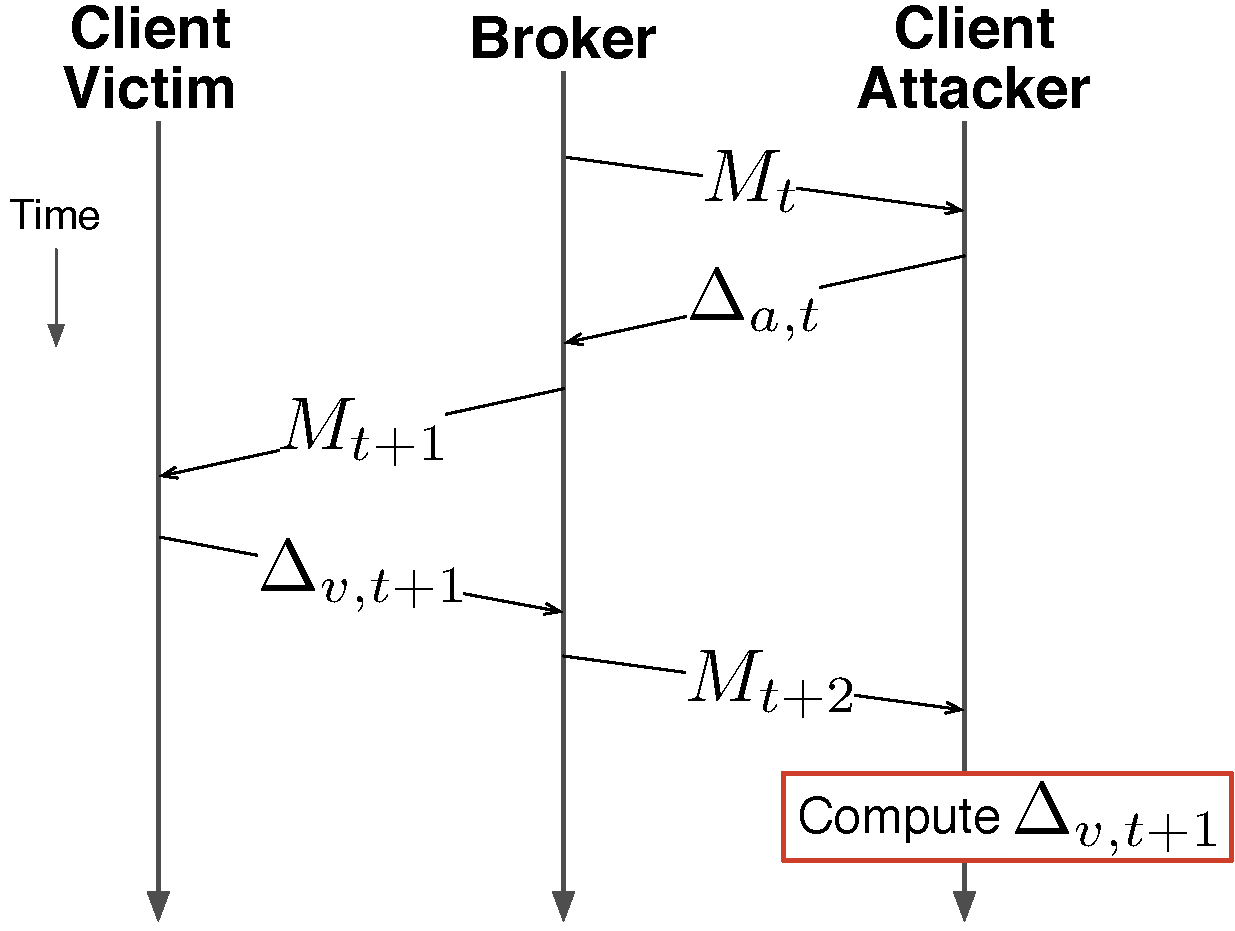
\includegraphics[width=.8\linewidth]{fig/inversionattack.pdf}
  \caption{One iteration in an inversion attack in which an attacker
    observes the difference between $M_t$ and $M_{t+2}$, and infers
    this difference to be $\Delta_{V,t+1}$. After many iterations,
    the attacker can discover $M^*_V$, the optimal model trained on
    the victim's data.}
  \label{fig:inversion-timespace}
\end{figure}

Although a direct inversion attack in federated learning has not
been realized yet, we envision a novel potential attack in this
scenario. Figure~\ref{fig:inversion-timespace} shows the proposed ideal
situation for an attacker performing an inversion attack: a two client
TorMentor system, one of whom is the adversary.

In this scenario the victim $V$ and attacker $A$ alternate in sending
gradient updates to the broker. Since the global model parameters are
sent to the adversary at each iteration, it can ideally observe the
difference in the global model between iterations. As the attacker
knows their contribution to the global model at the previous
iteration, they are able to exactly compute the victim's update by
calculating:
\begin{align*}
  M_{t+2} &= M_t + \Delta_{v,t+1} + \Delta_{a,t} \\
  \Delta_{v,t+1} &= M_{t+1} - M_t - \Delta_{a,t}
\end{align*}
By saving and applying $\Delta_{v,t}$ at each iteration to a hidden,
shadow model, the adversary can compute an approximation to $M_V$,
the optimal model trained with only the victim's data, similar to a
model stealing attack~\cite{Tramer:2016}. The adversary can then
perform a model inversion attack~\cite{Fredrikson:2014,
Fredrikson:2015} and reconstruct the victim's training data elements
in $X_V$. In the case that the broker carries out the inversion attack,
the attack is even stronger: the broker can isolate all updates sent to
it through a single connection.

Differential privacy offers a natural defense against attacks from a
broker or another client by perturbing the victim's updates $\Delta_
{V,t}$ that are sent to the broker. An adversary will find it difficult
to recover $M_V$ and $X_V$ when the privacy parameter $\varepsilon$ is
closer to 0. An adversary could choose to send any vector as their
$\Delta_{a,t}$ update, which allows them to curate specific gradients
that elicit revealing responses from the victim~\cite{Hitaj:2017}.

In the case of attacks from other clients, the effectiveness of
the differentially private SGD protocol is also contingent on a setting
in which multiple clients are simultaneously performing updates. When
an adversarial client receives a new copy of the global model in
TorMentor, it has no mechanism to discover which clients contributed to
the model since the last update, making it difficult to derive
knowledge about specific clients in the system. 

Thus, TorMentor exposes a privacy parameter $k$ to clients, which
clients use to express the minimum number of clients that must be in
the system before training can begin. Our differentially private SGD
only begins when $n$ clients, each with a parameter $k \le n$ exist in
the system. Effectively, this means that for an adversarial client to
perform the ideal model inversion against a victim with parameter $k$
the adversary needs to create $k-1$ sybil clients.

\section{Defending against poisoning attacks}
\label{validator}

\begin{algorithm}[t]
  \KwData{Stream of gradient updates from each client $i$, over $t$
  iterations $\Delta_{i,t}$}
  \KwResult{Reject a client if their updates oppose the defined
  learning objective}
  \While{IsTraining} {
    Draw Bernoulli value $v$\;
    \If{$v > \mathit{VALIDATION\mbox{\tt\string_}RATE}$} {
      Set current model $M_t$ to be snapshot model $M_s$\;
      Wait for client responses\;
    }
    \If{Client $c$ contacts TorMentor} {
      Send $M_s$ instead of $M_t$\;
      Save response $\Delta_{c,s}$
    }
    \If{All clients responded} {
       Find RONI $r_c$:
       $r_c = err(M_s, X_{val}) - err(M_s + \Delta_{c,s}, X_{val})$\; 
       $total_c = total_c + r_c$\;
      \If{$total_c > \mathit{THRESHOLD}$} {
        penalize $c$\;
      }
    }
  }
  \caption{RONI validation algorithm. \label{alg:roni}}
\end{algorithm}

In adding the validator process, we propose an \emph{active parameter
server} alternative to the assumed passive parameter server in current
attacks~\cite{Hitaj:2017}. The parameter server validates each client's
contribution to the model health and penalizes updates from suspicious
connections. 

We develop a distributed RONI defense that uses sets of gradient
updates, instead of datasets, and independently evaluates the influence
that each gradient update has on the performance of a trusted global
model. Validation (Algorithm~\ref{alg:roni}) executes within the
parameter server in TorMentor and validates that iterations performed
by clients have a positive impact. Validation is parameterized by two
variables: the validation rate at which validations are performed, and
the RONI threshold~\cite{Barreno:2010} required before a client is
flagged.

To ensure that validations are performed in a fair manner, we benchmark
all clients against the same candidate model. The validator
intersperses validation iterations within the gradient updates requests
in distributed SGD. A validation round is triggered through a periodic 
Bernoulli test, with the probability parameterized by a validation
rate. During a validation round, the current model state is
snapshotted, and a copy of this model is sent to all active clients.
The clients' gradient responses are collected and the RONI value is
calculated and accumulated. 

In addition to the proof of work required to join the system, we
implement an adaptive proof of work mechanism to mitigate sybils in
poisoning attacks. A SHA-256 proof of work puzzle that must be solved
on each iteration before an update to the global model is accepted by
the broker. When a client's RONI score exceeds a defined negative
threshold, the broker increases the required trailing number of 0's by
one, increasing the difficulty of the puzzle for that client. The
difficulty of this puzzle is client- and iteration-specific, making it
more expensive for malicious clients to poison the model and decreasing
their influence relative to honest clients. 

When the rate of validation is increased, the broker discovers
poisoning clients more quickly, but with a performance overhead. When
the RONI threshold is increased, the broker is more likely to detect
adversaries, but the false positive rate of flagging honest nodes
increases as well.

An important design detail is that a validation request looks just
like a gradient update request. Therefore, adversaries cannot
trick the validator by appearing benign during validation rounds while
poisoning the true model. If the snapshot model $M_s$ is taken close
enough to the current model state $M_t$, it becomes more difficult for
adversaries to distinguish whether the updates they are receiving are
genuine gradient requests or not.

\section{Modular design}

To summarize, TorMentor includes several mechanisms to provide
various levels of client and curator privacy and security. These
include:
\begin{itemize}[label=$\star$]
    \item Using Tor to provide anonymous communication for all users 
    (clients and the curator).
    \item Using proof of work as a form of admission control.
    \item A validator process that uses RONI and adaptive proof of work
        to mitigate poisoning attacks and sybils.
    \item Differentially private SGD and minimum client enforcement to
        provide client privacy and to defend against inversion attacks.
\end{itemize}

Each of these components operates independently, and if brokered
learning is deployed in a setting where some of the described attacks
are out of scope, these components can be independently disabled. %%  in the
%% system.
